
\section{Proceso de pentesting} 

\subsection{¿que es un prueba de penetración o pentest?}
Según la definición de OWASP \autocite{web1} un test de penetración o pentesting, a veces denominado 
prueba de caja negra, es esencialmente el arte de probar
un sistema o aplicación para descubrir vulnerabilidades de seguridad, sin conocer el funcionamiento interno de la mismas. Normalmente el equipo 
encargado de las pruebas de penetración accede a las aplicaciones como si fuesen usuarios. El pentester tratará con 
que ese nivel de acceso encontrar vulnerabilidades que se puedan explotar en la aplicación.

El propósito de la prueba de penetración es determinar la presencia 
de vulnerabilidades potencialmente explotables y analizar el impacto de estas,
sí se detecta alguna. La mejor forma de probar una defensa es tratando de penetrar en ella.
\newpage

\subsection{Fases del prueba de intrusión}
A la hora de realizar una prueba de intrusión o pentest distinguimos las siguientes fases, basándonos en 
la distinción realizada en pentesting con Kali  \autocite{ref1};  dicjhas fases son las siguientes:
\begin{itemize}
    \item Alcance y términos de la prueba de intrusión.
    \item Recolección de información.
    \item Análisis de vulnerabilidades.
    \item Explotación de vulnerabilidades.
    \item Postexplotación del sistema.
    \item Generación de informes.
\end{itemize}
\subsubsection{Alcance y términos de la prueba de intrusión.}  
Para esta fase normalmente se genera un documento de plan de pruebas. En muchos casos es 
necesaria la revisión y aprobación de dicho documento por parte del dueño del sistema a probar 
(\gls{sut}), antes de poder comenzar con el proceso de pentesting.
    En dicho documento de pruebas se suel detallar la siguiente información:
    \begin{itemize}
        \item Sistema sobre el que se realizan las pruebas.
        \item Los tipos de prueba a realizar.
        \item Herramientas que se van a utilizar.
        \item Proceso de seguimiento de los defectos encontrados.
        \item Documentos que se entregarán durante el proceso de pentesting.
        \item Restricciones en la ejecución de la prueba de intrusión
    \end{itemize}

\subsubsection{Recolección de información.}
Una vez definido el plan de pruebas procederemos a recolectar información 
del sistema o aplicación indicado en dicho plan. 
        
Principalmente obtendremos información mediante los procesos de enumeración y 
análisis de código que detallaremos en el siguiente capítulo. 

\subsubsection{Análisis de vulnerabilidades.}
Al finalizar los procesos anteriores se analizarán los defectos encontrados para descartar falsos positivos y 
después se hará entrega un reporte de análisis dinámico con los defectos no descartados. 
Para cada uno de los defectos detectados que se incluyan en el reporte abriremos defecto en el sistema de gestión de defectos.

\subsubsection{Explotación de vulnerabilidades.}

En el caso de que uno o varios defectos necesiten ser explotados, y siempre solicitando permiso se detallará 
el proceso de explotación indicando las herramientas y \glspl{exploit} necesarios para realizar este proceso. 
En este proceso también se deben detallar las consecuencias, si las hubiese de la ejecución de las herramientas y 
exploits a utilizar sobre la aplicación o sistema objetivo.

\subsubsection{Postexplotación del sistema.}

En este caso también es necesario solicitar permiso al dueño del sistema, detallando 
la forma en que persistirá el ataque en la aplicación o sistema objetivo.

\subsubsection{Generación de informes.}

Llegados a este punto ya se deben haber hecho entrega de los reportes del análisis estático, si se dispone de acceso al código fuente, y del reporte de análisis dinámico. Sí se ejecutasen los procesos de explotación o Postexplotación se ampliaría el reporte de análisis dinámico con la información recabada en dichos procesos.

A parte de los reportes anteriores, se debe entregar un informe de resultado de 
pruebas con el resultado de ejecución del proceso de pentest incluyendo en 
el mismo el detalle de los defectos reportados en el sistema de gestión de 
defectos, si es posible, así como el estado en que se encuentran en el momento
de entrega de dicho reporte.

\newpage
\section{Herramientas de enumeración}

El proceso de enumeración trataremos de recabar información de recurso accesibles del sistema 
o aplicación. Para este proceso existen númerosas utilidades, entre las más utilizadas estarían:

\begin{itemize}
    \item Nmap:     Utilizada para el escaneo de puertos
    \item Nikto:    Utilizada para recopilación de recursos disponibles.
    \item Dirb:     Utilizada para recopilación de recursos disponibles.
    \item TestSSL:  Utilizda para la revisión de certificados y mecanismos de cifrado SSL.
\end{itemize}

\newpage
\section{Herramientas de análisis de código}

Detro de los procesos actuales de \gls{ssdlc} cada vez cobran más importacia la inclusion de herramientas de analisis de codigo durante el proceso de desarrollo del Software.

Dentro de las herramientas de análisis de código, podemos hacer la siguietne distinción:

\begin{itemize}
    \item \textbf{Herramientas de Análisis de código estático (\Gls{sast}).} 
    El análisis estático es un proceso que se realiza sobre el código de una aplicación 
    sin necesidad de ejecutarse.

    El  análisis de código estático, también conocido como Análisis de código fuente \Gls{sca}, 
    realiza pruebas sobre el código fuente para la detección temprana de defectos en dicho código. El uso de este
    tipo de herramientas es recomendable realizarlos en la fase de implementación del ciclo
    de desarrollo seguro  \gls{ssdlc}.

    \item \textbf{Herramientas de análisis de código Dinámico (\Gls{dast}.)} 
    Este tipo de análisis se realiza sobre una aplicación o servicio desplegado y en ejecución, a diferencia del tipo anterior.

    En análisis DAST enviará peticiones maliciosas al sistema objetivo para verificar la presencia de diversos tipos de ataques.

        
    \item \textbf{Herramientas híbridas.} 
    Las herramientas hibridas son aquellas que presentan proceso para definir los dos tipos de análisis anteriores.
\end{itemize}
    

\subsection{Herramientas de análisis estático de código}

La metodología  \gls{owasp} \gls{asvs} 4.0 se introdujo una sección para añadir 
los controles de codigo fuente como un requisito más dentro 
de la lista de requerimientos  para un desarrollo seguro:

\begin{figure}[h!]  
    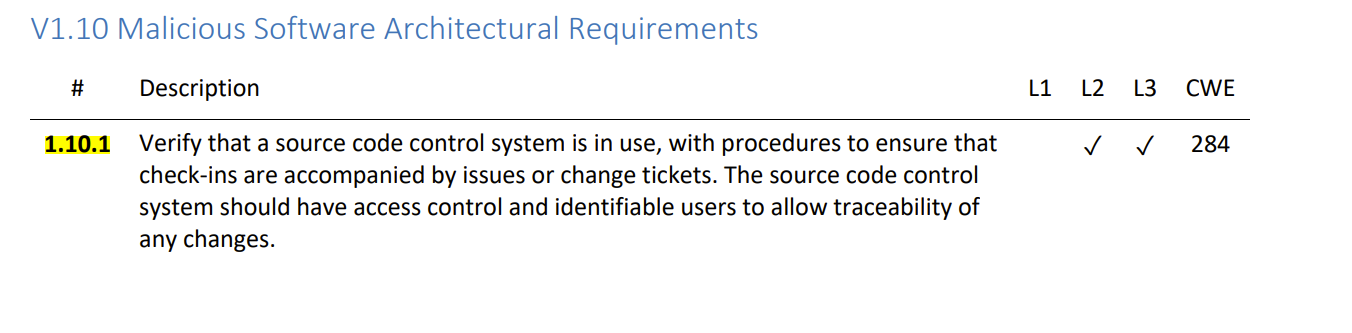
\includegraphics[width=\linewidth]{./imagenes/01_OWASP Application Security Verification Standard 4.0.png}
    \caption{ASVS 4.0 10.0.1 Security control.}  
    \label{fig:ASVS 4.0}
\end{figure}

Actualmete en mucho de los ciclos de desarrollo estas herramientas se encuentran integradas dentro de los procesos de Integración 
continua (\gls{ci}) y despliegue continuo (\gls{cd}), esto permite que ante cualquier cambio en el código se ejecuten estas
herramientas de forma automática permitiendo que ante cualquier cambio se ejecuten este tipo de herramientas de forma 
automática en los procesos de compilación y despliegue. 

También es común que las herramientas de análisis de código estén integradas dentro de los IDEs de desarrollo; lo cual permite 
que los desarrolladores también puedan hacer uso de estas herramientas y mejorar la calidad del código antes de su entrega.

Entre las distintas herramientas de análisis, para la implementación de nuestra infraestructura de pruebas haremos uso 
de las siguientes herramientas:
\begin{itemize}
    \item SonarQube
    \item Dependency-check
\end{itemize}
\newpage

\subsubsection{SonarQube}
Es una plataforma de para el análisis estático de código, dispone de distintos escáneres para la mayor parte de 
lenguajes de programación. Entre las versiones disponibles de SonarQube, podemos hacer uso de la 
versión \emph{“Community”} que es de uso libre.

\begin{figure}[h!]  
    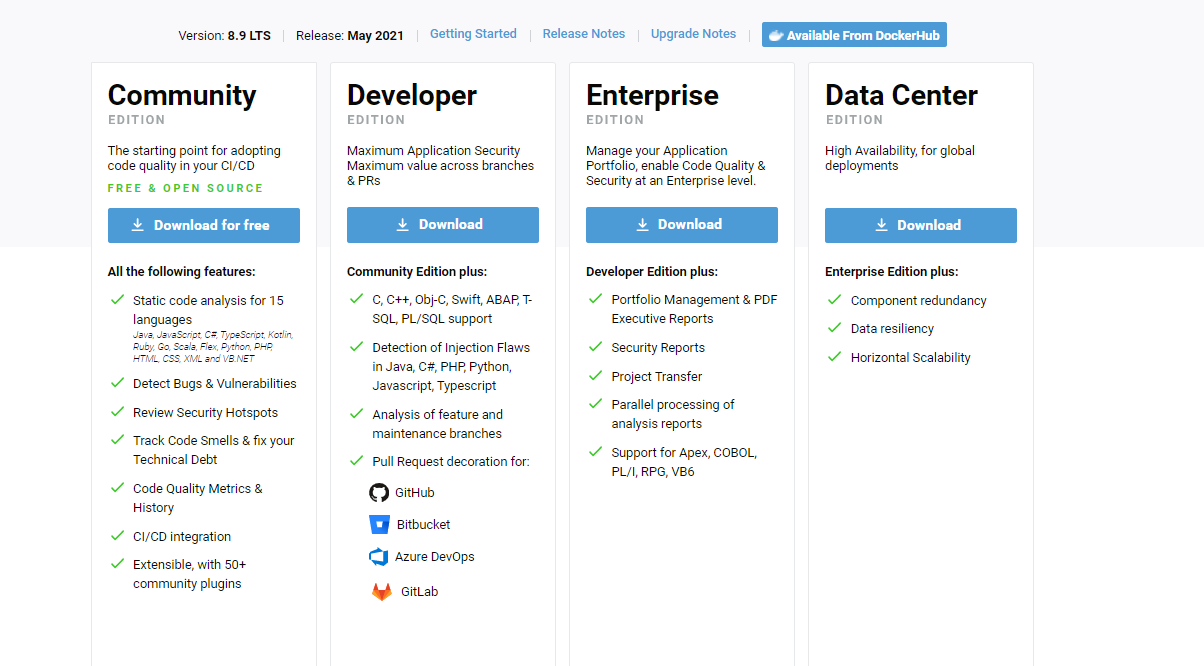
\includegraphics[width=\linewidth]{./imagenes/02_SonarQubeEditions.png}
    \caption{Versiones Sonarqube 8.9.}  
    \label{fig:logo}
\end{figure}

La versión \emph{“Community”} incluye escáneres para los siguientes lenguajes de programación:

\begin{multicols}{2}
    \begin{itemize}
        \item Java
        \item JavaScript
        \item c\#
        \item TypeScript
        \item Ruby
        \item Go
        \item Scala
        \item Flex 
        \item Python
        \item PHP
        \item HTML 
        \item CSS
        \item XML
        \item VB.Net
    \end{itemize}
\end{multicols}

Además, mediante extensiones de la comunidad podemos añadir escáneres para los siguientes lenguajes:

\begin{itemize}	
    \item PL\\SQL
    \item C\\C++
\end{itemize}    

\subsubsection{Dependency-check}
Es una herramienta de análisis de dependencias que intenta detectar vulnerabilidades divulgadas públicamente contenidas en las dependencias de 
un proyecto. Para ello, determina si existe un identificador de enumeración de plataforma común (CPE) para una dependencia determinada. Si lo encuentra, generará
un informe vinculado a las entradas \gls{cve} asociadas.

Actualmente OWASP Dependency-Check puede analizar dependencias de proyectos Java y .Net, que se encuentran totalmente soportados otros lenguajes como Ruby, Node.js, 
PHP (composer), Swift Package Manager y Python tienen un soporte más limitado.

El componente de análisis de dependencias de OWASP Dependency-Check puede ser ejecutado de las siguientes formas:

\begin{itemize}
    \item Ant task
    \item \href{https://github.com/jeremylong/DependencyCheck/releases/download/v6.1.6/dependency-check-6.1.6-release.zip}{Command Linet Tool}
    \item Grandle plugin
    \item \href{https://search.maven.org/#artifactdetails%7Corg.owasp%7Cdependency-check-maven%7C6.1.6%7Cmaven-plugin}{Maven plugin}
    \item SBT plugin
\end{itemize}

El uso de dependency-check desde la línea de comandos tiene los siguientes parámetros principales:

begin{table}
  \begin{center}
  \caption{Parámetros línea comandos dependency-check}
  \label{tab:tabla 1}
  \begin{tabular}{c|c}
    \textbf{Parámetro} & \textbf{Descripción}\\
    \hline
      --project & Especifica el nombre del proyecto que aparecerá en el reporte.\\ 
      --scan & Directorio donde se encuentran las librerías de terceros.\\
      --out &  Directorio de salida del reporte de análisis de dependencias.\\
      --suppresion & Fichero .xml que contiene vulnerabilidades que deben de ser excluidas del reporte 
      (falsos positivos)      
  \end{tabular}
\end{center}
\end{table}
Ejemplo de uso:\\
\begin{verbatim}
  dependency-check.bat 
      --project "juice-shop" 
      --scan "D:\CodigoAnalisis\Seguridad\juice-shop\node_modules" 
      --out "D:\CodigoAnalisis\Seguridad\WebGoat.NET\reports" 
\end{verbatim}

\subsection{Herramientas de análisis dinámico de código}
Para las ejecuciones de análisis dinámico haremos uso de la herramienta Zed Attack Proxy (ZAP) de OWASP en su versión 2.10. OWASP Zap es una de las herramientas de 
software para análisis dinámico de aplicaciones que es mantenida y distribuida por la organización \href{https://owasp.org/www-project-zap/}{OWASP}. Su principal objetivo es el 
análisis de seguridades en aplicaciones web orientados a empresas, se caracteriza por ser de código abierto y totalmente gratuita.\\

La Interfax de OWASP ZAP Desktop está compuesta de los siguientes elementos:
\begin{figure}[h!]  
    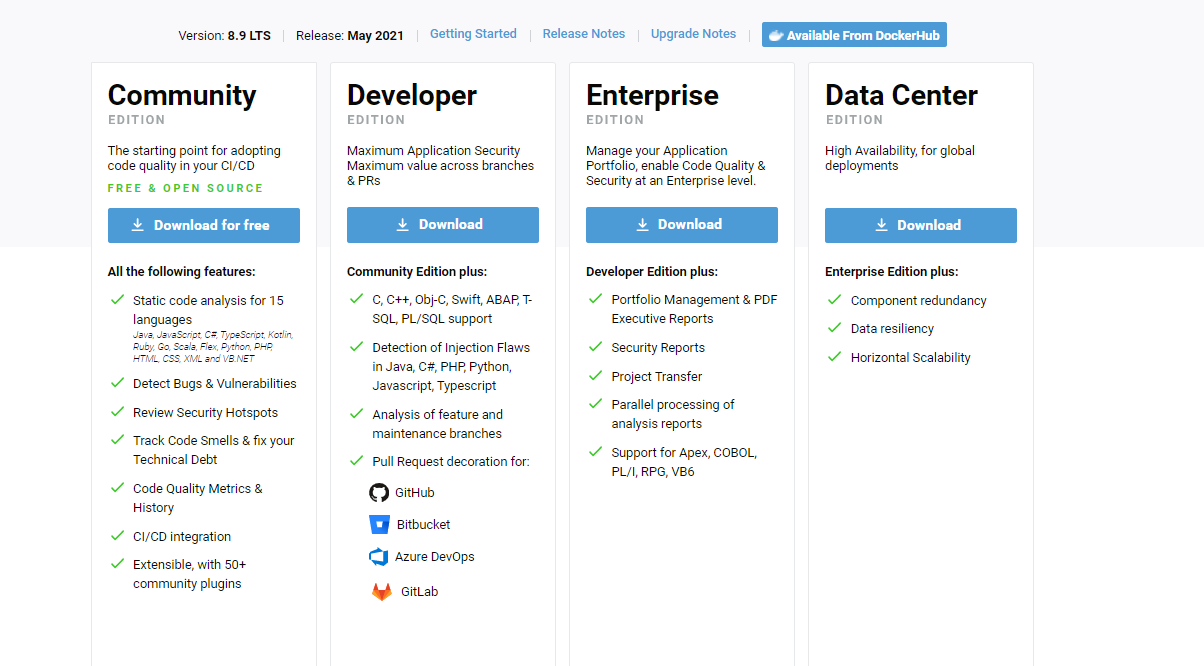
\includegraphics[width=\linewidth]{./imagenes/02_SonarQubeEditions.png}
    \caption{Interfaz OWASP Zap}  
    \label{fig:Interfaz OWASP Zap}
\end{figure}

\begin{itemize}
    \item \textbf{Barra menú:} Proporciona acceso a las funcionalidades manuales y automáticas de la aplicación.
    \item \textbf{Barra herramientas:} Incluye botones de acceso rápido a las funciones más comunes.
    \item \textbf{Panel vista árbol:} Muestra los sitios visitados, así como los scripts utilizados.
    \item \textbf{espacio de trabajo:} Muestra las peticiones y respuestas de las peticiones y permite editarlas.
    \item \textbf{Ventana de in formación:} Muestra los detalles de las herramientas automáticas y manuales utilizadas. 
    \item \textbf{Pie} Muestra el resumen de alertas encontradas por los distintos escáneres realizados.
\end{itemize}

Para más información consultar documentación, \href{https://www.zaproxy.org/docs/desktop/ui/}{ver documentación ZAP UI}

A la hora de ejecutar el análisis dinámico haremos uso de las siguientes políticas de pruebas 
que serán ejecutados en cada una de las iteraciones para cada aplicación o sistema objetivo:

\begin{itemize}
    \item \textbf{Escáner regular:} Para ampliar las rutas válidas dentro de los dominios a evaluar más allá de la utilizadas en sesión de pruebas utilizada.
    \item \textbf{Escaner Completo:} A partir del resultado del escáner regular, donde se ampliará la batería de pruebas a realizar.
\end{itemize}